\documentclass[12pt,a4paper]{article}
\usepackage[utf8]{inputenc}
\usepackage{geometry}
\geometry{a4paper, margin=1in}
\usepackage{hyperref}
\usepackage{graphicx}
\usepackage{tabularx}
\usepackage{enumitem}
\usepackage{tikz}
\usetikzlibrary{shapes.geometric, arrows.meta, positioning}

\title{\textbf{Medical ERP System} \\ Methodology \& System Design Report}
\author{}
\date{\today}

\begin{document}

\maketitle

\section{Introduction}
\textbf{The Medical ERP System} is a comprehensive, multi-role medical enterprise resource planning (ERP) system designed to streamline pathology and hospital management operations. Built using robust Java Enterprise technologies, the platform facilitates efficient patient management, diagnostic test tracking, real-time internal communication, and automated patient notifications via WhatsApp.

\section{Development Methodology}
The development of the system followed an \textbf{Agile and Iterative} methodology, ensuring continuous integration of features such as real-time chat and third-party API integrations without disrupting core functionalities.

\subsection{Architectural Pattern}
The application strictly adheres to the \textbf{Model-View-Controller (MVC)} design pattern, promoting a clean separation of concerns:
\begin{itemize}[leftmargin=*]
    \item \textbf{Model}: Represents the data structures (e.g., Users, Patients, Tests) and the Data Access Objects (DAOs) responsible for database transactions.
    \item \textbf{View}: The presentation layer responsible for rendering the UI and capturing user inputs using JSP and Bootstrap 5.
    \item \textbf{Controller}: Java Servlets act as controllers, intercepting HTTP requests, invoking the appropriate business logic (Services), and routing data to the correct JSP views.
\end{itemize}

\subsection{Technology Stack}
\begin{itemize}
    \item \textbf{Frontend}: HTML5, Vanilla CSS, Bootstrap 5, Vanilla JavaScript.
    \item \textbf{Backend Application}: Java (JDK 17+), Jakarta EE (Servlets, JSP, WebSockets).
    \item \textbf{Database}: MySQL 8.0+.
    \item \textbf{Server}: Apache Tomcat 10+.
    \item \textbf{External Integrations}: Meta WhatsApp Cloud API / Twilio (for SMS/WhatsApp alerts).
\end{itemize}

\section{System Architecture}
The application operates on a classic \textbf{3-Tier Architecture} tailored for scalable web applications.

\subsection{Presentation Layer}
\begin{itemize}
    \item Utilizes responsive web design principles.
    \item Client-side validation using JavaScript before payload submission.
    \item WebSocket client implementation for instant messaging.
\end{itemize}

\subsection{Business Logic (Application Layer)}
\begin{itemize}
    \item \textbf{Servlet Controllers}: Handle traditional synchronous requests (e.g., login, form submissions).
    \item \textbf{WebSocket Endpoints}: Maintain persistent, bi-directional connections for real-time chat between staff members.
    \item \textbf{Service Classes}: Encapsulate complex logic, such as constructing HTTP requests to the WhatsApp API.
\end{itemize}

\subsection{Data Access Layer}
\begin{itemize}
    \item Utilizes raw JDBC (Java Database Connectivity) via custom DAO classes (e.g., \texttt{ChatDAO}, \texttt{PatientDAO}).
    \item A centralized \texttt{DBConnection} class manages the database connection pool securely.
\end{itemize}

\section{Database Design}
The relational database is normalized to maintain data integrity.

\subsection{Entity-Relationship (ER) Diagram}
\begin{figure}[h]
    \centering
    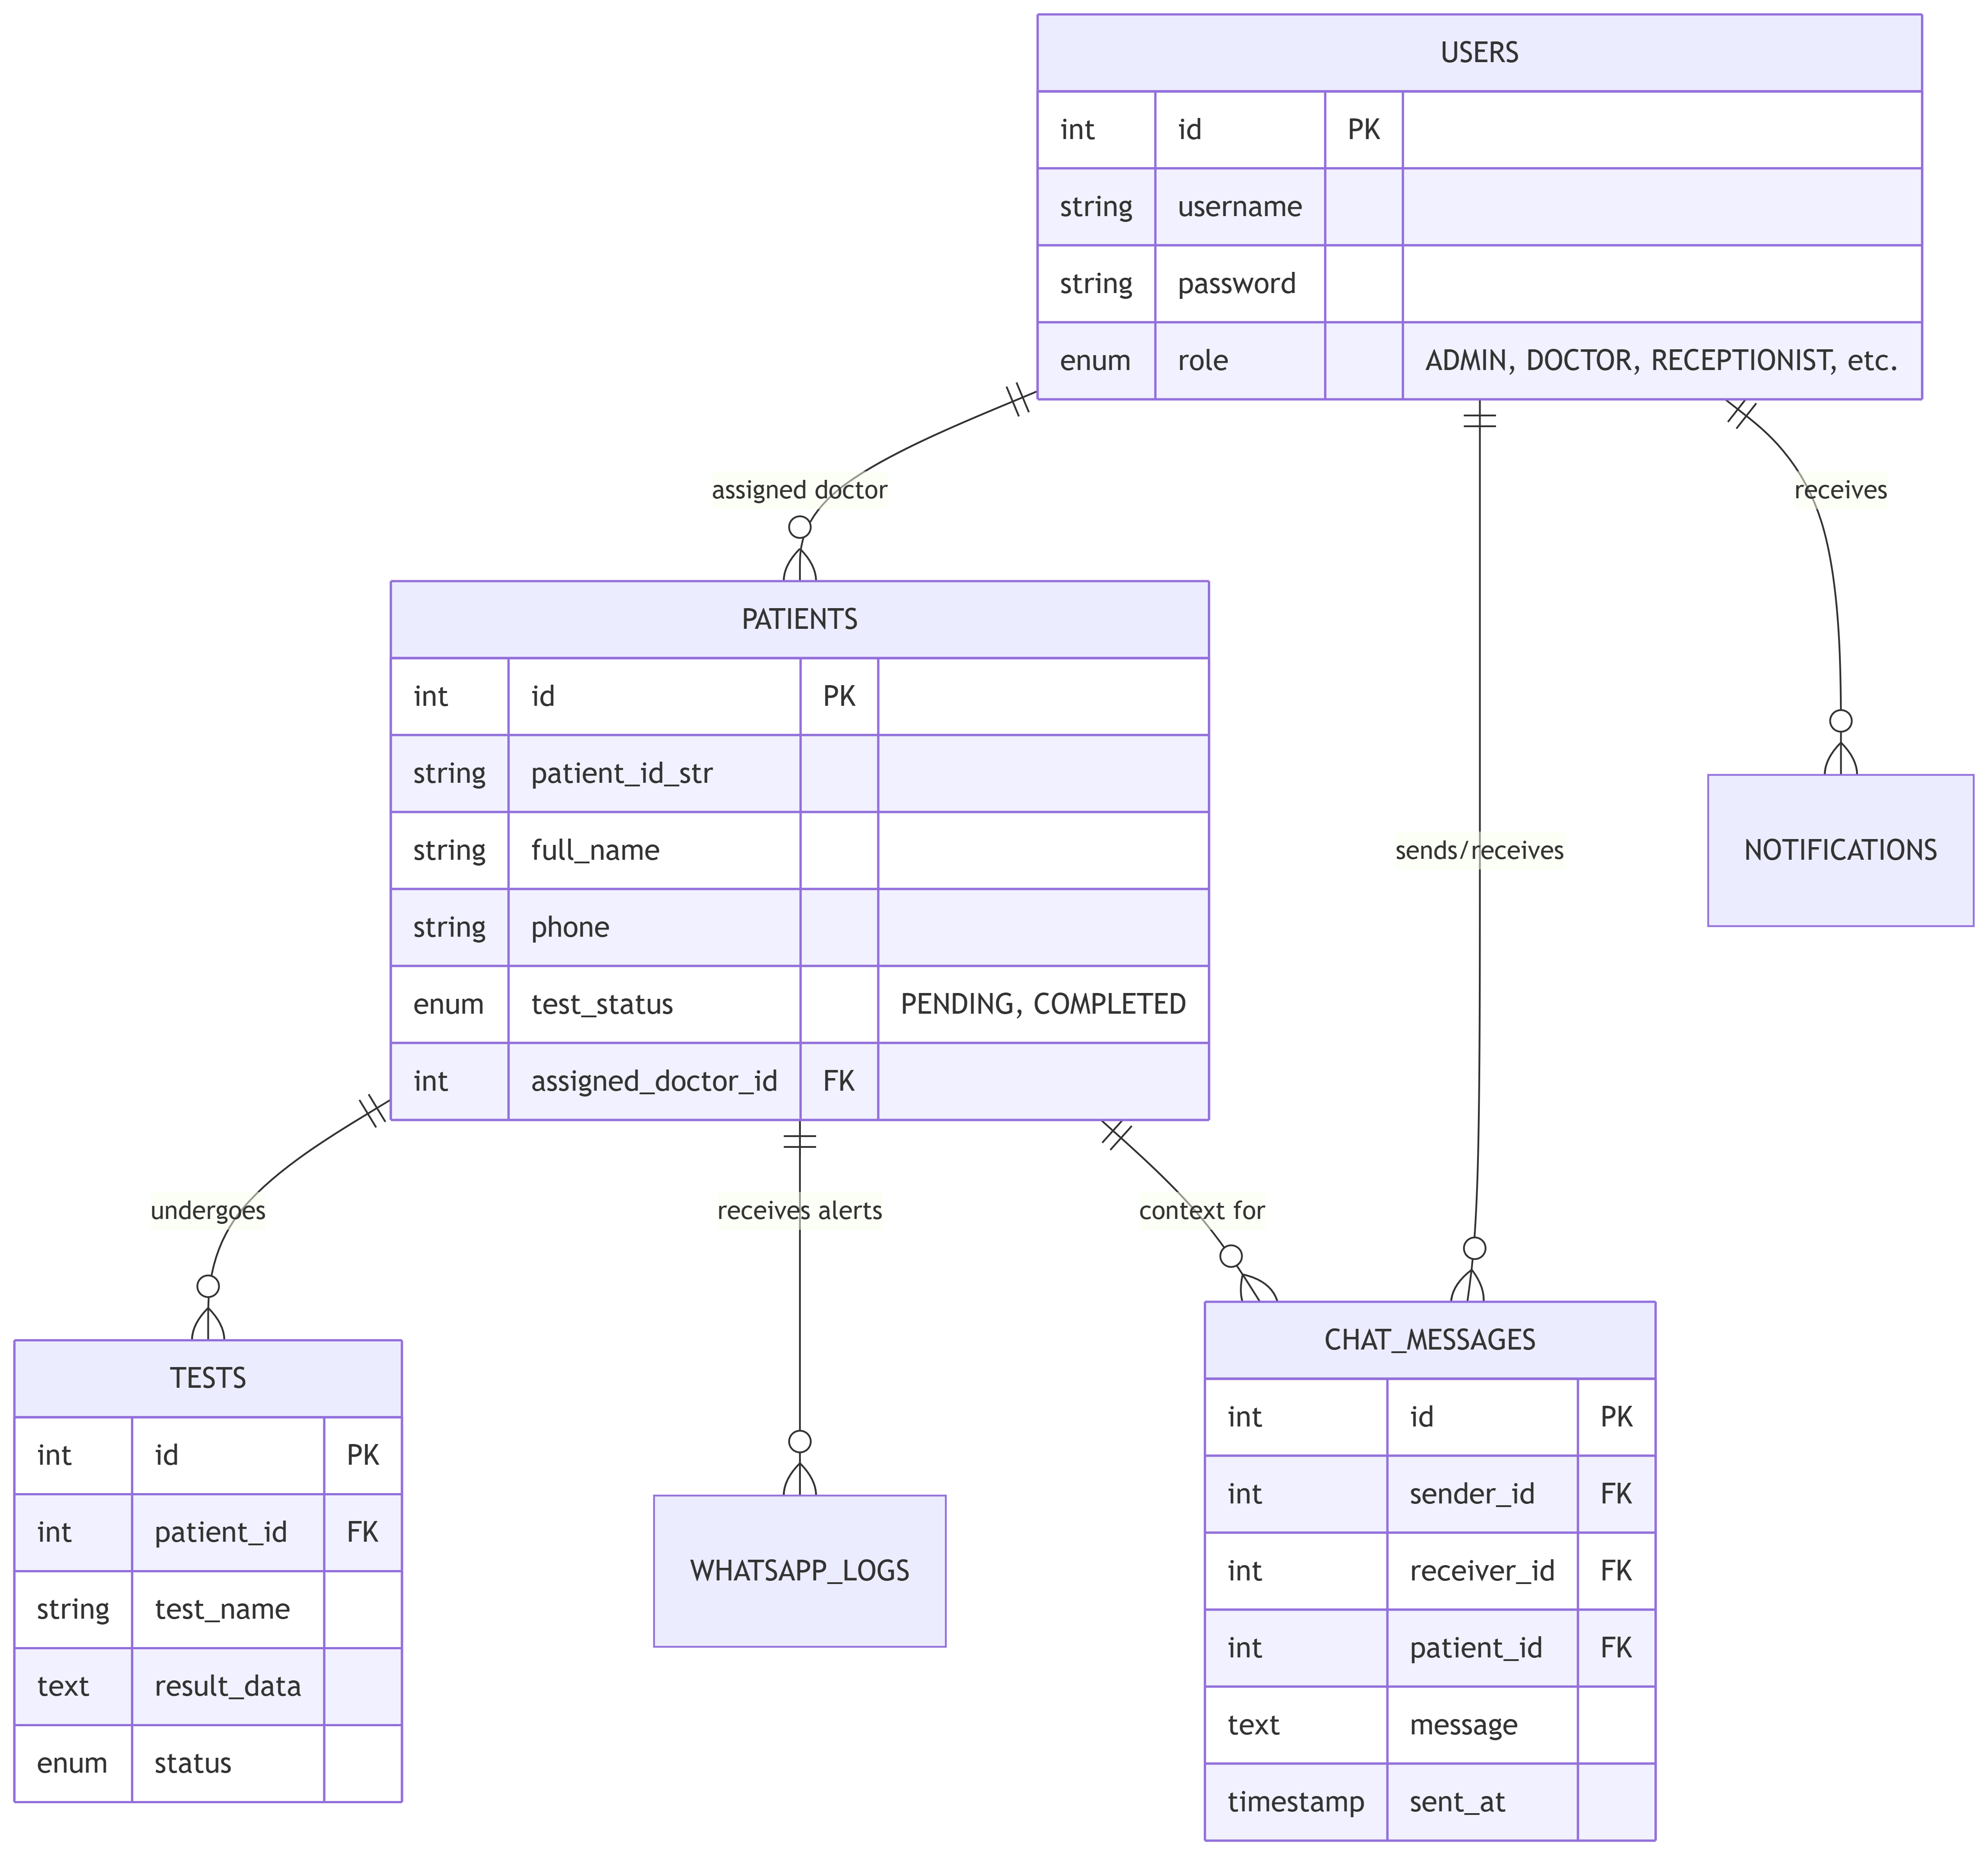
\includegraphics[width=\textwidth]{db.png}
    \caption{Database Schema Overview}
    \label{fig:er_diagram}
\end{figure}

\subsection{Core Entities}
\begin{enumerate}
    \item \textbf{Users}: Central to Role-Based Access Control (RBAC). Differentiates between Admins, Doctors, Psychologists, Lab Staff, and Receptionists.
    \item \textbf{Patients}: Stores demographic data and tracks the overall lifecycle/status of their investigation.
    \item \textbf{Tests}: Links to patients and stores raw diagnostic result data.
    \item \textbf{Chat Messages}: Stores historical chat data, linking the sender, receiver, and optionally the \texttt{patient\_id} if the chat pertains to a specific case.
\end{enumerate}

\section{Key Modules and Workflows}

\subsection{Role-Based Access Control (RBAC)}
\begin{itemize}
    \item \textbf{Authentication}: Users log in via a central portal. Passwords should be hashed before storage.
    \item \textbf{Authorization}: HTTP Sessions and Servlet Filters restrict access. For example, only a user with the \texttt{LAB\_STAFF} role can update test results, while \texttt{RECEPTIONIST} can register new patients.
\end{itemize}

\subsection{Real-Time Communication (WebSocket)}
To facilitate seamless collaboration without page refreshes, a WebSocket server is implemented.
\begin{enumerate}
    \item Staff connects to the WebSocket server upon logging in.
    \item Messages are routed through the session manager and simultaneously persisted to the database via \texttt{ChatDAO}.
    \item Offline messages are stored and fetched upon the user's next login.
\end{enumerate}

\subsection{Automated WhatsApp Notifications}
\begin{itemize}
    \item Integrated via the \texttt{WhatsAppService}.
    \item Triggered asynchronously when critical database events occur (e.g., updating a test status from \texttt{PENDING} to \texttt{COMPLETED}).
    \item All outbound communication is logged in the \texttt{whatsapp\_logs} table for auditing and debugging API delivery failures.
\end{itemize}

\section{Future Enhancements \& Scalability}
While the current monolithic architecture is highly effective for a single hospital deployment, future iterations could adopt:
\begin{itemize}
    \item \textbf{Connection Pooling}: Migrating from raw JDBC to HikariCP for better database performance under heavy load.
    \item \textbf{ORM Integration}: Using Hibernate/JPA to replace raw SQL queries in DAOs, reducing boilerplate code.
    \item \textbf{Microservices}: Decoupling the WebSocket chat and WhatsApp notification workers from the main Tomcat instance to scale them independently.
\end{itemize}

\end{document}
